\documentclass[11pt,a4paper]{article}
\usepackage[margin=2.4cm]{geometry}
\usepackage{amsmath,amssymb}
\usepackage{graphicx}
\usepackage{booktabs}
\usepackage[hidelinks]{hyperref}
\usepackage{microtype}
\usepackage{enumitem}

\newcommand{\vj}{v_j}
\newcommand{\vi}{v_i}
\newcommand{\Wij}{W_{ij}}
\newcommand{\Eij}{E_{ij}}
\newcommand{\msg}{\mathrm{msg}}
\newcommand{\act}{\mathrm{act}}

\title{Circuit parameter extraction}
\author{}
\date{}

\begin{document}
\maketitle



\section{Generator vs GNN}

The generator is a conductance-based network of $N$ neurons. For neuron $i$,
%
\begin{equation}
\tau_i \frac{d\vi}{dt}
   \;=\; -\bigl(\vi - V^{\mathrm{rest}}_i\bigr) \;+\; \msg_i \;+\; I_i ,
\qquad
\msg_i \;=\; \sum_{j \in \mathcal{N}(i)} \Wij \,\act(\vj)\,\bigl(\Eij - \vi\bigr),
\label{eq:gen}
\end{equation}
%
with $\act = \mathrm{relu}$ on this data, $\Wij \ge 0$ a synaptic conductance in
units of the leak conductance, and $\Eij$ the reversal potential of the channel
the presynaptic cell opens. The sign of a synapse lives entirely in the driving
force $\Eij - \vi$, never in $\Wij$.

The model is a graph network with the same connectivity:
%
\begin{equation}
\frac{d\vi}{dt} \;=\; f_\theta\!\bigl(\vi, a_i, \widehat{\msg}_i, I_i\bigr),
\qquad
\widehat{\msg}_i \;=\; \sum_{j \in \mathcal{N}(i)} \widehat{W}_{ij}\;
     g_\phi\!\bigl(\vj, a_j, \vi, a_i\bigr),
\label{eq:model}
\end{equation}
%
where $a_i$ is a learned per-neuron embedding and $\widehat{W}_{ij}$ a learned
per-edge weight. Only $d\vi/dt$ is supervised. \emph{Nothing in the loss observes
$\widehat{\msg}$}, and that is the whole difficulty: the message is an internal
variable, and any transformation of it that $f_\theta$ can undo leaves the
training objective exactly unchanged. We suppose that the model's message is
related to the truth by
%
\begin{equation}
\widehat{\msg}_i \;=\; \frac{1}{k_i}\,\msg_i \;+\; \beta_i .
\label{eq:gauge}
\end{equation}
%
Write the model's update in the same form as the generator's, which is what
the update fit of \S\ref{sec:update} measures:
%
\begin{equation}
\frac{d\vi}{dt} \;=\; T_i\Bigl[\bigl(V_i - \vi\bigr) + G_i \widehat{\msg}_i
                              + f(I_i)\Bigr].
\label{eq:updatetmpl}
\end{equation}
%
Substituting \eqref{eq:gauge} into \eqref{eq:updatetmpl} and expanding puts the
model's update in terms of the true message,
%
\begin{equation}
\frac{d\vi}{dt} \;=\; -\,T_i\,\vi
   \;+\; \frac{T_i G_i}{k_i}\,\msg_i
   \;+\; T_i\bigl(V_i + G_i \beta_i\bigr)
   \;+\; T_i f(I_i),
\label{eq:updateexpanded}
\end{equation}
%
while the generator \eqref{eq:gen}, divided by $\tau_i$ and grouped the same way,
reads
%
\begin{equation}
\frac{d\vi}{dt} \;=\; -\,\frac{1}{\tau_i}\,\vi
   \;+\; \frac{1}{\tau_i}\,\msg_i
   \;+\; \frac{V^{\mathrm{rest}}_i}{\tau_i}
   \;+\; \frac{I_i}{\tau_i}.
\label{eq:genexpanded}
\end{equation}
%
The two hold for every trajectory the network produces, so the coefficients of
$\vi$, of $\msg_i$ and the constant must agree one by one. Matching them gives
three identities:
%
\begin{align}
\text{message:} && T_i G_i \frac{1}{k_i} &= \frac{1}{\tau_i}
   &&\Longrightarrow&& k_i = \tau_i\, T_i\, G_i ,
   \label{eq:kid}\\[2pt]
\text{leak:}    && T_i &= \frac{1}{\tau_i}
   &&\Longrightarrow&& \tau_i = 1/T_i ,
   \label{eq:tauid}\\[2pt]
\text{constant:}&& T_i V_i + T_i G_i \beta_i &= \frac{V^{\mathrm{rest}}_i}{\tau_i}
   &&\Longrightarrow&& V^{\mathrm{rest}}_i = \tau_i T_i V_i + k_i \beta_i .
   \label{eq:vrestid}
\end{align}
%
\section{The readout, as least squares}
\label{sec:readout}

With the identities in hand the question becomes an empirical one: does the
trained network obey the generator's equation~\eqref{eq:gen} at all, and if so
with which constants? The two are answered by the same fit. Impose the
generator's form on what the network computes, ask least squares for the
constants that fit it best, and read the residual: the coefficients are the
recovered parameters, and the $R^2$ is how well the hypothesis holds on that edge
or that neuron. An edge whose message cannot be written as
$\Wij\,\act(\vj)\,(\Eij-\vi)$ reports a low $R^2$ and its constants mean nothing;
one that fits at $0.999$ has a message the generator could have produced, and
then the only question left is whether the constants are the right ones.


\subsection{Per edge: $\Wij$ and $\Eij$}
\label{sec:edge}

Write $u_t = \act(\vj(t))$. The generator's synaptic form, multiplied out, is
%
\begin{equation}
\msg_{ij}(t) \;=\; \Wij\,u_t\,\bigl(\Eij - \vi(t)\bigr) + C_{ij}
  \;=\; \underbrace{(\Wij \Eij)}_{b_1}\,u_t
  \;+\; \underbrace{(-\Wij)}_{b_2}\,\bigl(u_t\,\vi(t)\bigr)
  \;+\; \underbrace{C_{ij}}_{b_3},
\label{eq:edgelin}
\end{equation}
%
linear in $(b_1,b_2,b_3)$. The target is the model's OWN per-edge message,
$\widehat{\msg}_{ij}(t)$, taken from its forward pass, so the fit asks what
constants the generator would need to produce what the network computes. Stack
the $n$ usable frames $t_1 \dots t_n$ of this edge into a design matrix $A$ and
the model's messages into $y$:
%
\begin{equation}
A \;=\;
\begin{pmatrix}
u_{t_1} & u_{t_1}\vi(t_1) & 1\\
u_{t_2} & u_{t_2}\vi(t_2) & 1\\
\vdots  & \vdots          & \vdots\\
u_{t_n} & u_{t_n}\vi(t_n) & 1
\end{pmatrix}
\in \mathbb{R}^{n\times 3},
\qquad
b = \begin{pmatrix} b_1\\ b_2\\ b_3\end{pmatrix},
\qquad
y = \begin{pmatrix}
\widehat{\msg}_{ij}(t_1)\\ \vdots\\ \widehat{\msg}_{ij}(t_n)
\end{pmatrix}.
\label{eq:design}
\end{equation}
%
The problem is $\min_b \lVert A b - y\rVert_2^2$, whose normal equations
$A^{\!\top}\!A\,b = A^{\!\top}y$ give
%
\begin{equation}
b \;=\; (A^{\!\top}\! A)^{-1} A^{\!\top} y ,
\qquad
\Wij = -b_2 , \qquad \Eij = -\,b_1/b_2 , \qquad C_{ij} = b_3 .
\label{eq:edgesolve}
\end{equation}
%
$A^{\!\top}\!A$ is $3\times3$ whatever $n$ is, and its six distinct entries are
sums over frames --- $\sum u^2$, $\sum u^2 \vi$, $\sum u$, and so on --- so the
frames stream and nothing of size $n_{\mathrm{edges}} \times n$ is ever held.
All $434{,}112$ edges are then solved together as a batch of $3\times3$ systems,
in seconds.

\paragraph{Which rows are usable.} Three unknowns, so eight rows are ample. A
row is \emph{usable} when the presynaptic cell is above the activity floor,
$u_t = \act(\vj(t)) > 0$; below it the row is $[0,\,0,\,1]$ and constrains only
the offset. Frames are drawn where the presynaptic cells are actually on, and a
second sample tops up the edges still short, so $99.6\%$ of the $434{,}112$ edges
are fitted.

\paragraph{Why $\Eij$ is the fragile one.} $\Wij$ is a coefficient; $\Eij$ is a
ratio of two, so its relative error is
$(\sigma_E/E)^2 \approx (\sigma_{b_1}/b_1)^2 + (\sigma_{b_2}/b_2)^2$ and diverges
as $b_2 \to 0$. And $b_2$ is small not when the synapse is weak but when the
postsynaptic voltage barely moves: if $\vi(t) \approx c$ over the usable frames
then $u_t \vi(t) \approx c\,u_t$, the two columns are nearly the same vector,
and only the combination $b_1 + c\,b_2$ is determined. The guard is a $t$-test
on that coefficient, from the same normal equations:
%
\begin{equation}
\mathrm{se}(b_2) = \sqrt{\hat\sigma^2 \bigl[(A^{\!\top}\!A)^{-1}\bigr]_{22}},
\qquad
t = \frac{|b_2|}{\mathrm{se}(b_2)},
\qquad
\Eij \;\text{kept only where } t \ge 3 .
\label{eq:gate}
\end{equation}
%
Everything below it is recorded as unidentified rather than dropped silently. On
the conductance run used throughout: $432{,}517$ of the $434{,}112$ edges are
fitted ($99.6\%$), and of those, $405{,}503$ clear the gate and report a reversal
($93.4\%$ of all edges).

\subsection{Per neuron: $T_i$, $V_i$, $G_i$}
\label{sec:update}

The same least-squares approach on the update. Taking $f(I)$ linear, \eqref{eq:updatetmpl}
expands to a four-column regression of the model's own $d\vi/dt$ on its own
inputs,
%
\begin{equation}
\widehat{\frac{d\vi}{dt}} \;=\; a_0 + a_1\,\vi + a_2\,\widehat{\msg}_i
                              + a_3\,I_i ,
\qquad
T_i = -a_1 ,\quad V_i = a_0/T_i ,\quad G_i = a_2/T_i ,
\label{eq:updatesolve}
\end{equation}
%
again $(A^{\!\top}\!A)^{-1}A^{\!\top}y$, now $4\times4$ per neuron and accumulated
over frames so nothing of size $N \times n_{\mathrm{frames}}$ is ever held. The
fit's $R^2$ is reported: it is how far the model's update is from affine in the
message, and a low value invalidates $T$, $V$ and $G$ together.

\subsection{From the fitted coefficients to the circuit}
\label{sec:gauge}

The two fits return numbers about the model: per edge $(b_1,b_2,b_3)$, per neuron
$(a_0,a_1,a_2,a_3)$, and from them $T_i$, $V_i$, $G_i$, $\Wij^{\mathrm{fit}}$,
$\Eij$, $C_{ij}$. The identities \eqref{eq:kid}--\eqref{eq:vrestid} are what turn
those into the generator's parameters, and they are used in this order:
%
\begin{align}
\text{\eqref{eq:tauid}} && \tau_i &= 1/T_i = -1/a_1
  && \text{the time constant, directly},\\[2pt]
\text{\eqref{eq:kid}}   && k_i &= \tau_i T_i G_i = G_i = a_2/T_i
  && \text{the message scale, which $\Wij$ is in units of},\\[2pt]
\text{\eqref{eq:vrestid}} && V^{\mathrm{rest}}_i &= \tau_i T_i V_i + k_i \beta_i
  && \text{the resting level, offset included}.
\end{align}
%
So $\tau$ comes straight out of the update fit, $\Wij$ needs the scale from
\eqref{eq:kid} applied to the edge fit, and $V^{\mathrm{rest}}$ needs the offset
that \eqref{eq:vrestid} says the update hid in it --- the two corrections below.
$\Eij$ needs neither.

\paragraph{$\Wij$: divide by the scale.} By \eqref{eq:kid} the message is in
units of $1/k_i$ with $k_i = \tau_i T_i G_i$, and the fitted $b_2$ inherits that,
so the weight in the generator's units is
%
\begin{equation}
\Wij^{\mathrm{corrected}} \;=\; k_i \; \Wij^{\mathrm{fit}}
  \;=\; \tau_i\,T_i\,G_i \; \bigl(-b_2\bigr),
\qquad \tau_i = 1/T_i \;\Rightarrow\; k_i = G_i ,
\label{eq:wcorr}
\end{equation}
%
where $\tau_i$ is the model's own, from \eqref{eq:tauid}. Without this the same
weights score $R^2 = -2.14$ where the corrected ones score $0.995$ --- the
uncorrected number is kept as \texttt{Wij\_R2\_uncorrected} so the difference is
visible rather than assumed.

\paragraph{$V^{\mathrm{rest}}$: add the offset back.} By \eqref{eq:vrestid} the
level the update fit reads is short by exactly the neuron's own incoming message
offset:
%
\begin{equation}
V^{\mathrm{rest},\,\mathrm{corrected}}_i
  \;=\; \underbrace{\tau_i T_i V_i}_{\text{from the update fit}}
  \;+\; \underbrace{k_i \beta_i}_{\textstyle \sum_{j} C_{ij}\ \text{from Stage 1}} ,
\label{eq:vcorr}
\end{equation}
%

\section{A worked example}

Figure~\ref{fig:panels} shows the readout applied to neuron $2895$ of a
conductance network trained at process noise $\sigma=0.05$ on the flyvis
connectome ($N = 13{,}741$ neurons, $434{,}112$ edges).

\begin{figure}[htbp]
\centering
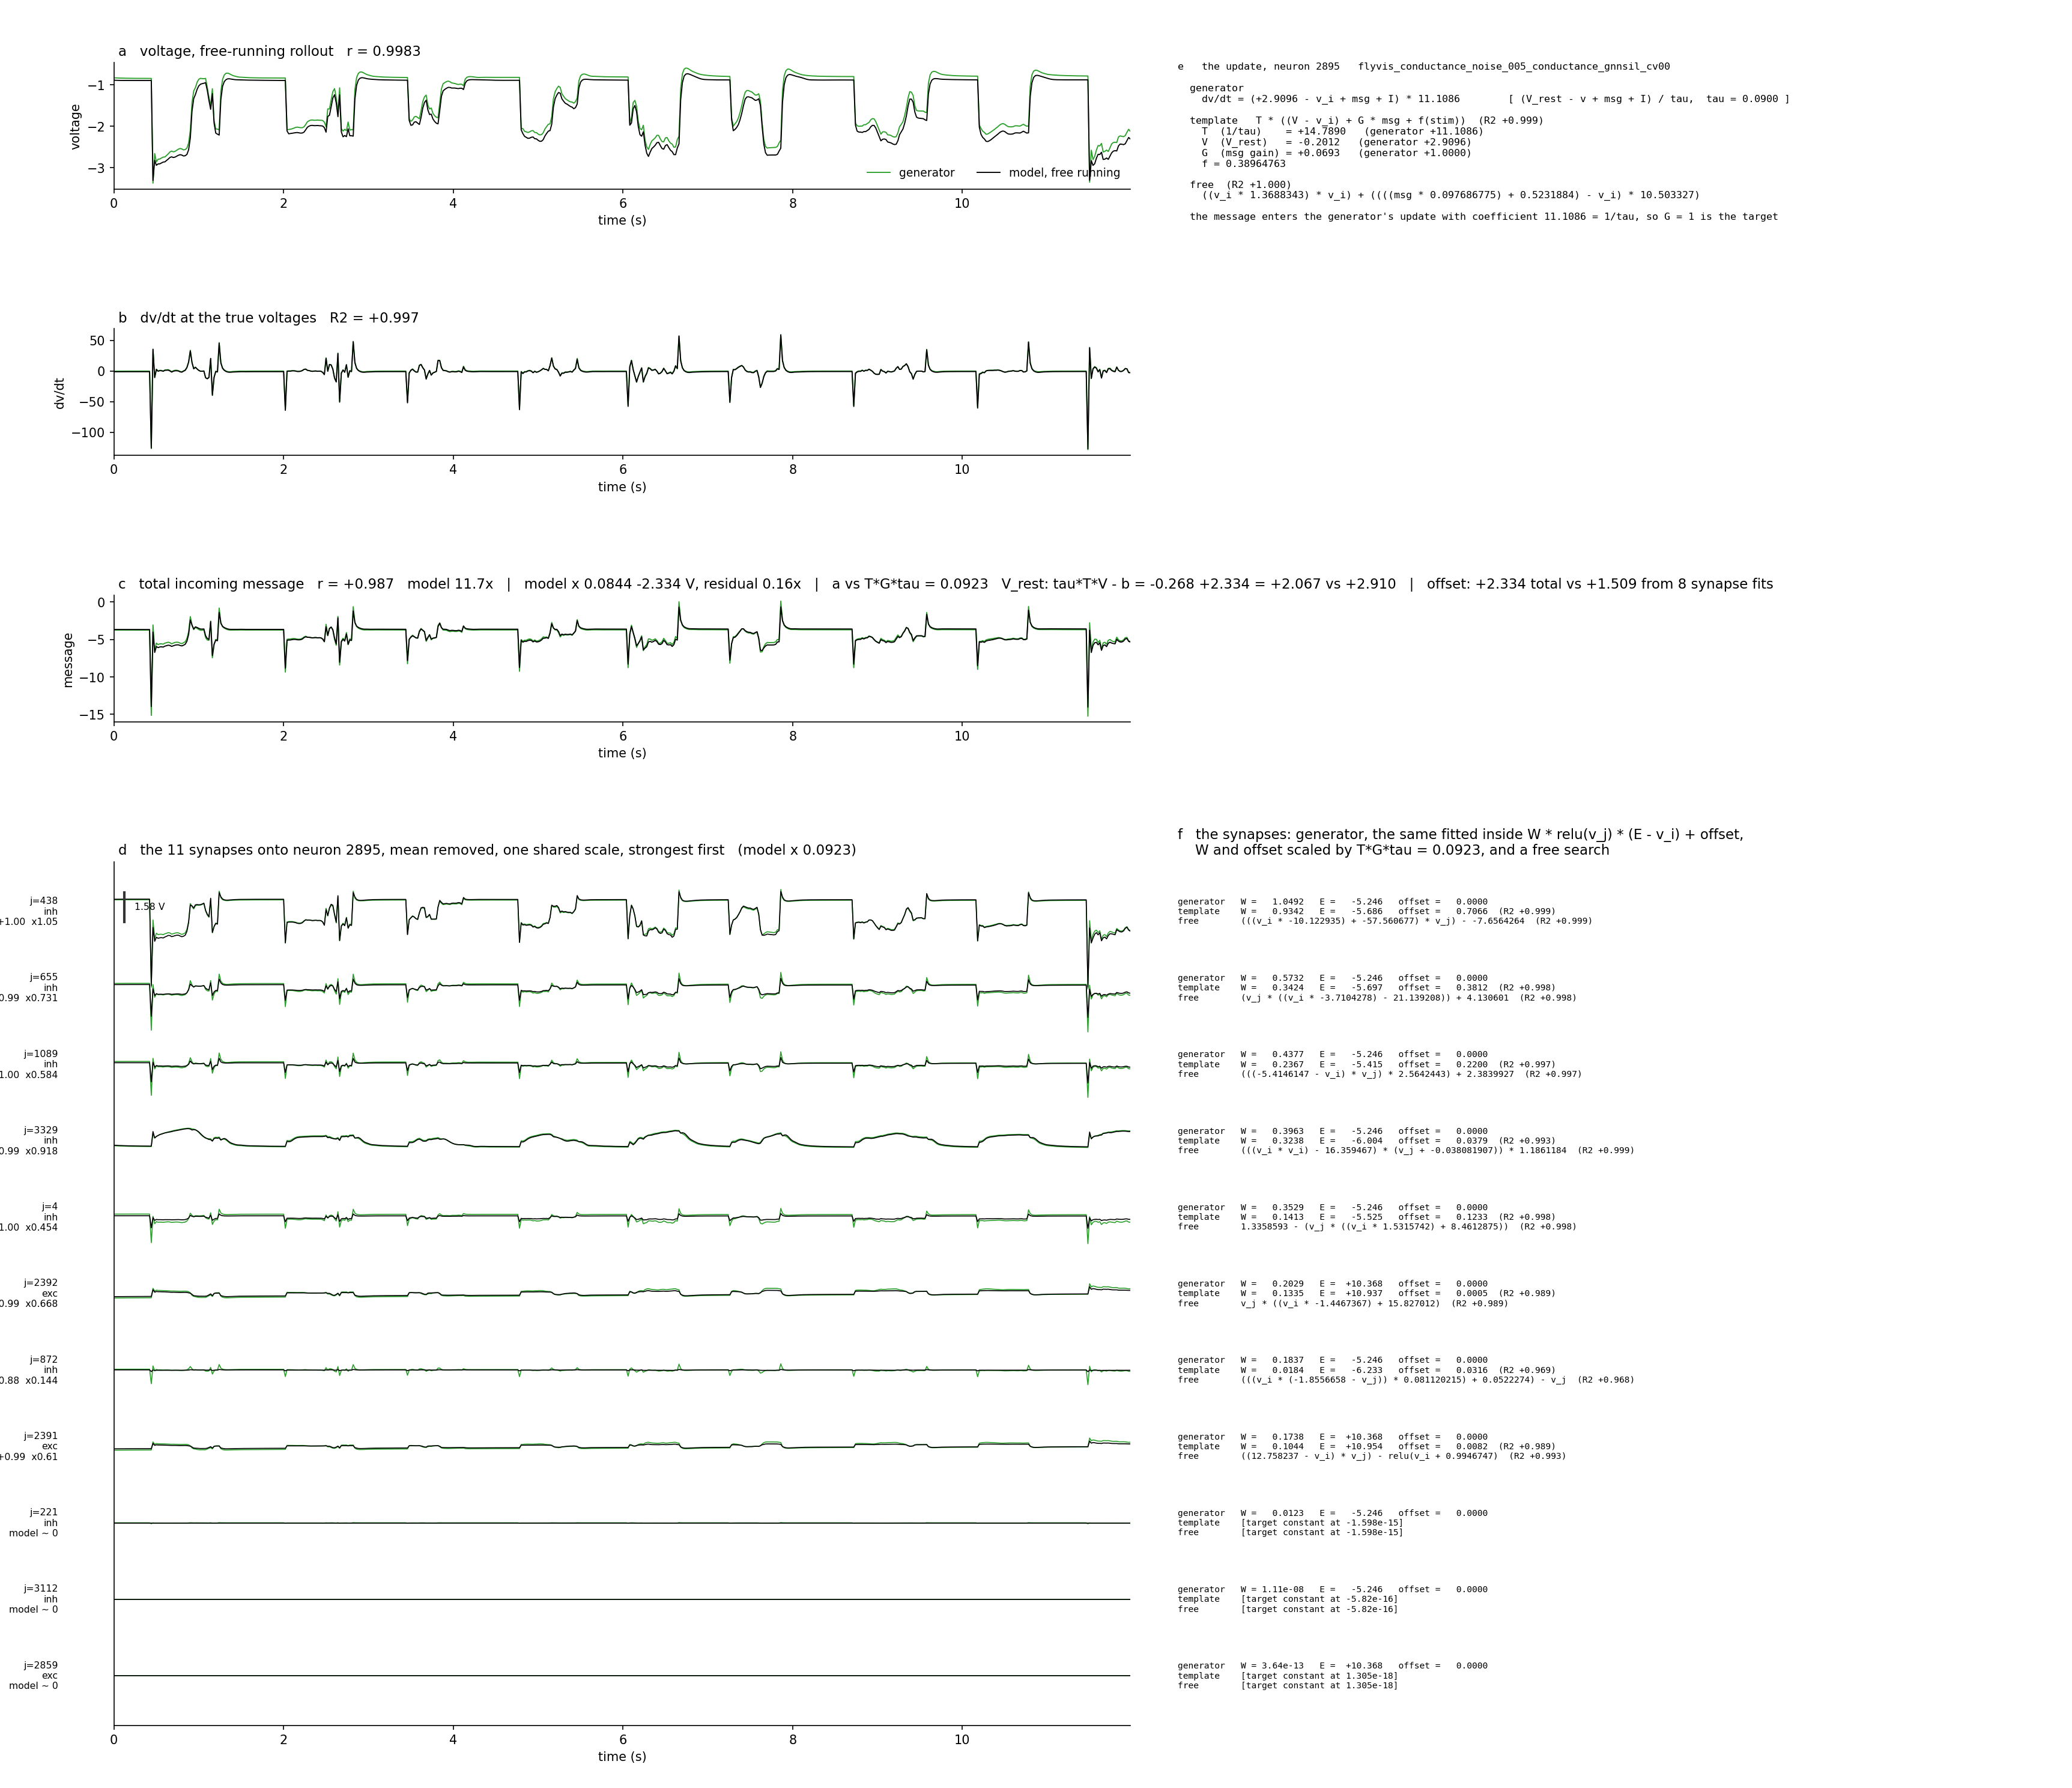
\includegraphics[width=\textwidth]{neuron2895_panels.png}
\caption{One neuron, term by term. \textbf{(a)}~free-running rollout, generator
in green and model in black, $r = 0.998$. \textbf{(b)}~$d v/dt$ at the true
voltages, $R^2 = 0.997$. \textbf{(c)}~the total incoming message: the learned one
after the affine correction of \eqref{eq:gauge}, against the generator's. The
heading reports the fitted scale $0.0844$ against $T G \tau = 0.0923$ from panel
(e) --- two independent routes to the same number, agreeing to $9\%$ --- and the
offset $b = -2.334$\,V. \textbf{(d)}~each of the $11$ synapses separately, mean
removed, on one shared voltage scale so that a synapse the model dropped looks
flat rather than being magnified to full height. \textbf{(e)}~the update fit of
\eqref{eq:updatesolve}: $T = 14.79$ against the generator's $1/\tau = 11.11$,
$G = 0.0693$ against a target of $1$. \textbf{(f)}~per synapse, the generator's
$(W, E, \text{offset}=0)$ against the template fit of \eqref{eq:edgesolve}, and a
free symbolic search for comparison.}
\label{fig:panels}
\end{figure}

\paragraph{The $V^{\mathrm{rest}}$ identity closes.} Equation~\eqref{eq:vrestid}
predicts $V^{\mathrm{rest}} = \tau T V - b$ where $b = -k\beta$ is the fitted
offset of panel (c). Substituting: $-0.083 + 2.334 = +2.251$ against the
generator's $+2.910$ --- $77\%$ of the resting potential recovered, of which
essentially all comes from the message's offset and almost none from the
update's own level $V = -0.21$. Reading $V$ alone as $V^{\mathrm{rest}}$, as a
naive fit of \eqref{eq:updatetmpl} invites, would be wrong by $3$\,V.

\paragraph{The per-edge offsets sum to the per-neuron one.} Panel (c) reports
$+2.334$ measured on the total message against $+1.510$ from summing the eight
fitted $C_{ij}$; the gap is the three synapses the model pruned, which have no
fit to contribute one. The two stages agree on a quantity neither of them
imposes.

\end{document}
